\chapter{Data}
\label{chap:datadescription}

\textcolor{red}{Jeg ville forslog at vi lavede en tabel ligesom i Regression med de værdier der mangler for de forskellige currencies for forskellige tenors, eller i hvert fald et overblik over hvad vi egentlig har data på - det er ikke den japanske yenn som mangler, tilbage fra 2004, der er ogsp manglende data på ander tenors}

This chapter describes the panel of par swap rates used to estimate and evaluate the affine-inspired arbitrage-free encoder--decoder framework. 

All data are obtained from Bloomberg and consist of quoted par swap rates reported in percentage terms. Prior to use, the rates are converted to decimal form. The data covers nine currencies,
\[
\{\text{AUD},\text{CAD},\text{DKK},\text{EUR},\text{GBP},\text{JPY},\text{NOK},\text{SEK},\text{USD}\}.
\]
observed at monthly frequency over the period 2004--2024. Table \textcolor{red}{INSERT A TABLE} summarizes the sample period and number of observations for each currency.

For each observation date, swap rates are available on the maturity grid
\[
\{1\text{Y},2\text{Y},3\text{Y},5\text{Y},7\text{Y},10\text{Y},15\text{Y},20\text{Y},30\text{Y}\}.
\]
Although the raw data contain swap rates at nine maturities, the model is fitted to the subset
\[
\{1\text{Y},2\text{Y},3\text{Y},5\text{Y},10\text{Y},15\text{Y},20\text{Y},30\text{Y}\},
\]
which corresponds to the maturity grid used in the encoder-decoder framework described in Section~\ref{chap:encoderdecodermodel}. The 7-year maturity is excluded to main consistency between the observed input data and the model specification.

The dataset exhibits substantial variation both across maturities and across currencies. Figure~\ref{fig:observed_curves} shows representative swap curves on 31 August 2016. Several features are apparent. First, most curves are upward sloping over short and intermediate maturities, while also displaying visible curvature over the full maturity spectrum. This pattern is consistent with the well-known result that a small number of factors can account for a large share of yield curve variation. Second, there are clear cross-currency differences in both level and shape. The Danish and euro curves are closely aligned across maturities, while the Japanese curve is noticeably lower and flatter than the others. Relative to the remaining currencies, the Japanese term structure also exhibits less pronounced curvature at medium and long maturities on this date.

\begin{figure}[H]
    \centering
    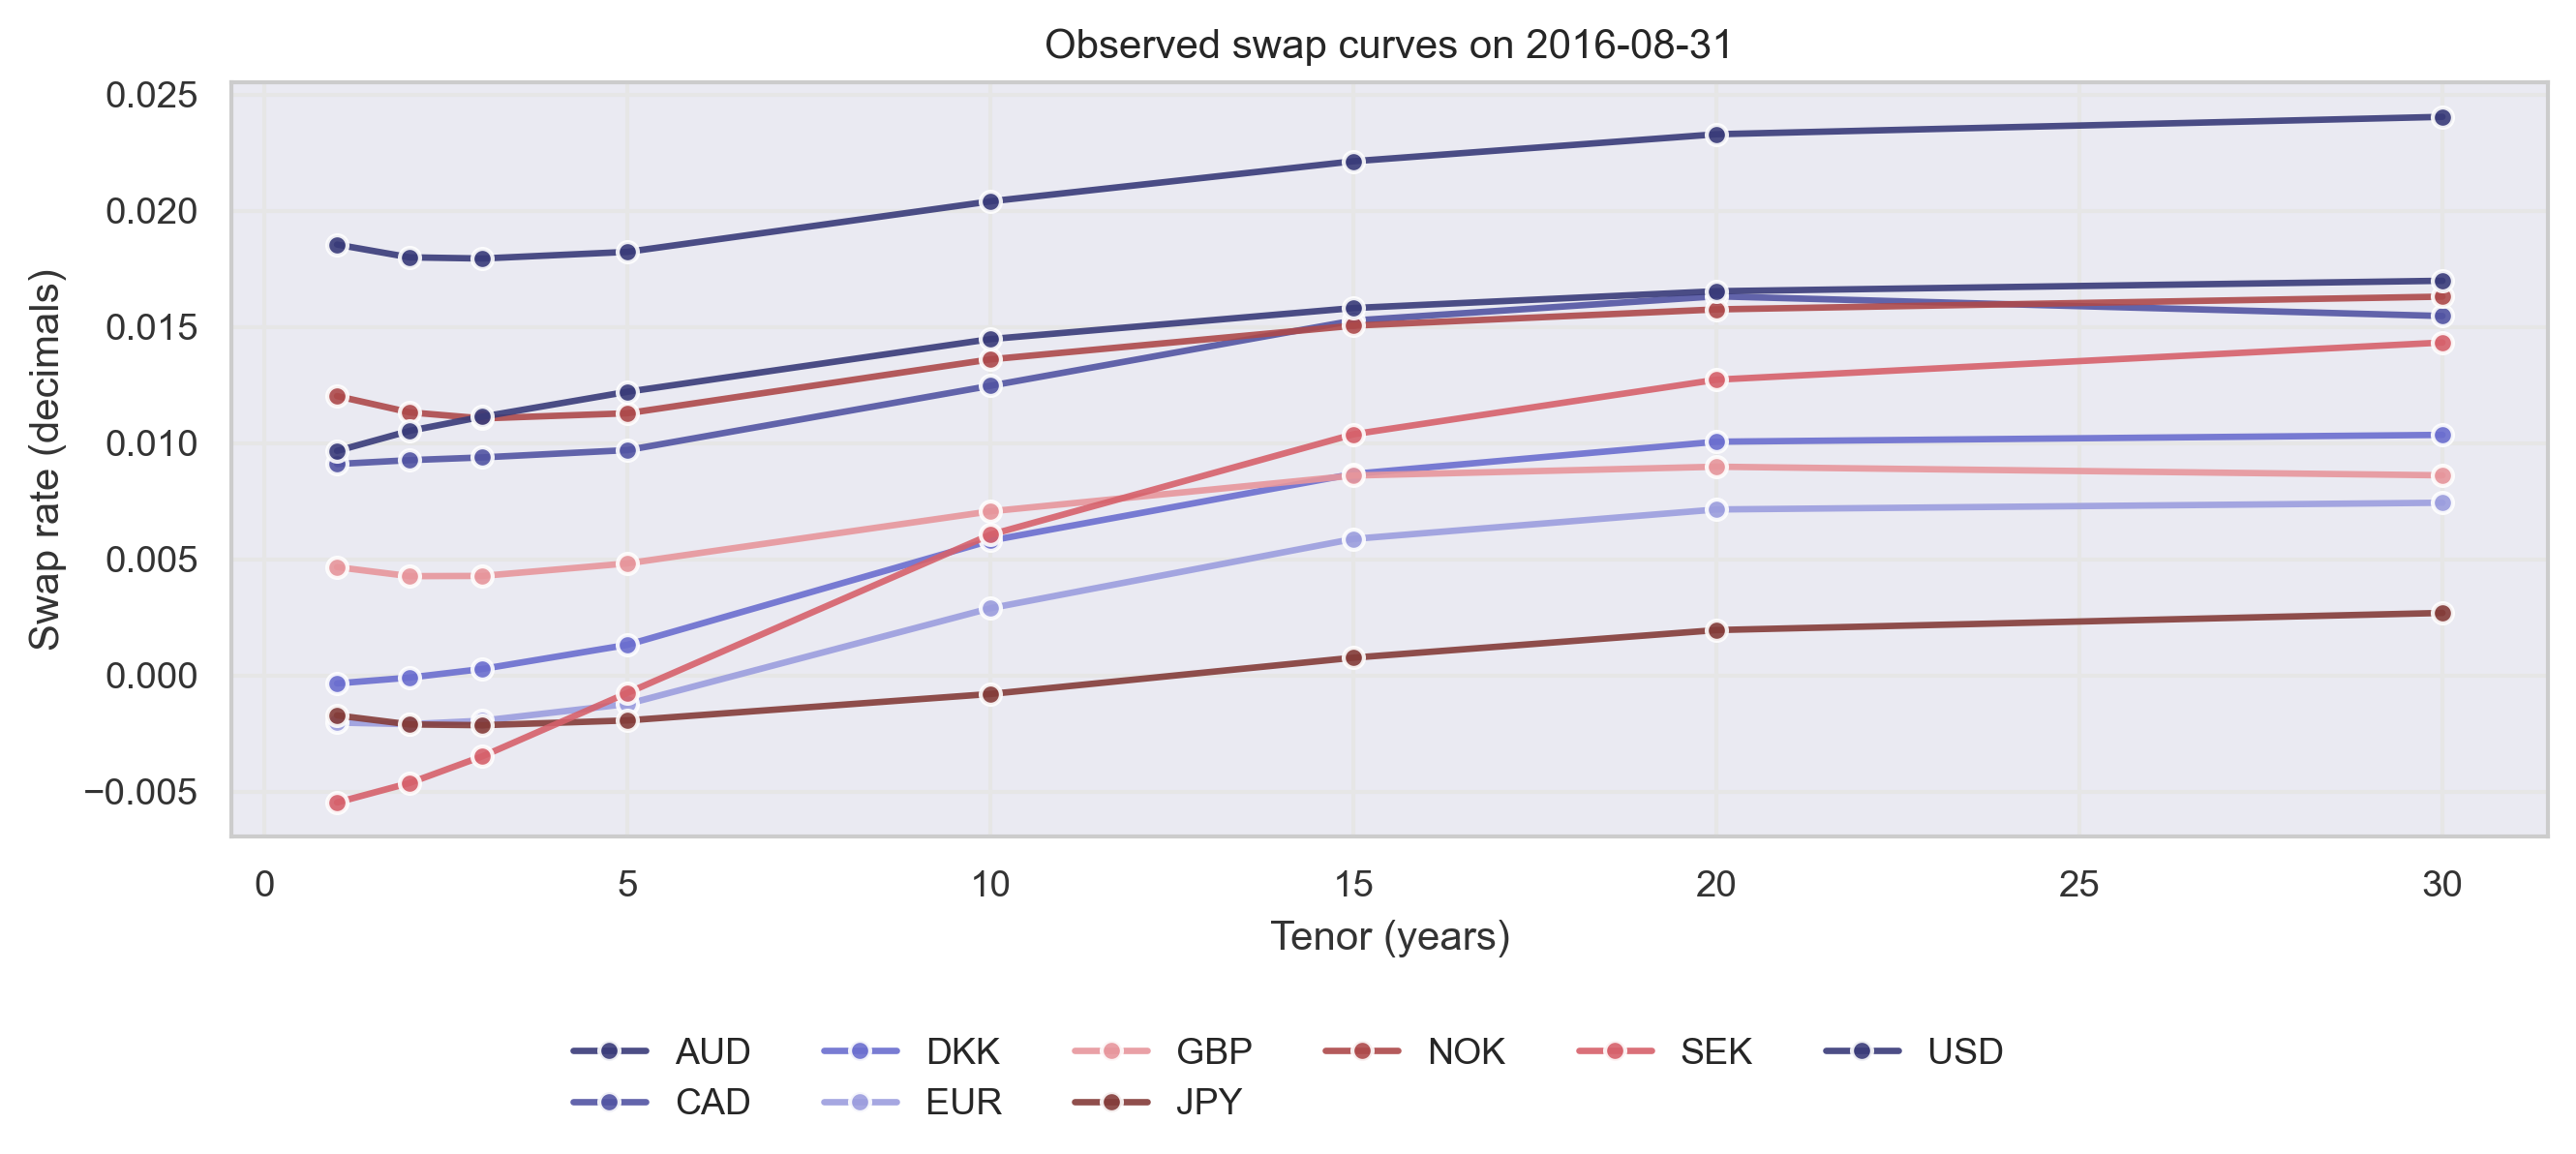
\includegraphics[width=0.9\textwidth]{Figures/bbg/paper_fig2a_observed_curves_2016-08-31_bbg.png}
    \caption{Observed swap curves across currencies on 31 August 2016.}
    \label{fig:observed_curves}
\end{figure}

These cross-sectional differences are complemented by substantial time-series variation. Figure~\ref{fig:timeseries_10y} plots the 10-year swap rate for each currency over the sample period and illustrates the evolution of long-term rates across different monetary environments. Long-term rates generally decline over the post-financial-crisis period and reach historically low levels around 2019--2020. From 2022 onward, however, rates rise sharply across most currencies. The sample therefore contains both prolonged low-rate regimes and periods of rapid monetary tightening, which makes it well suited for evaluating model performance across markedly different term-structure environments.

\begin{figure}[H]
    \centering
    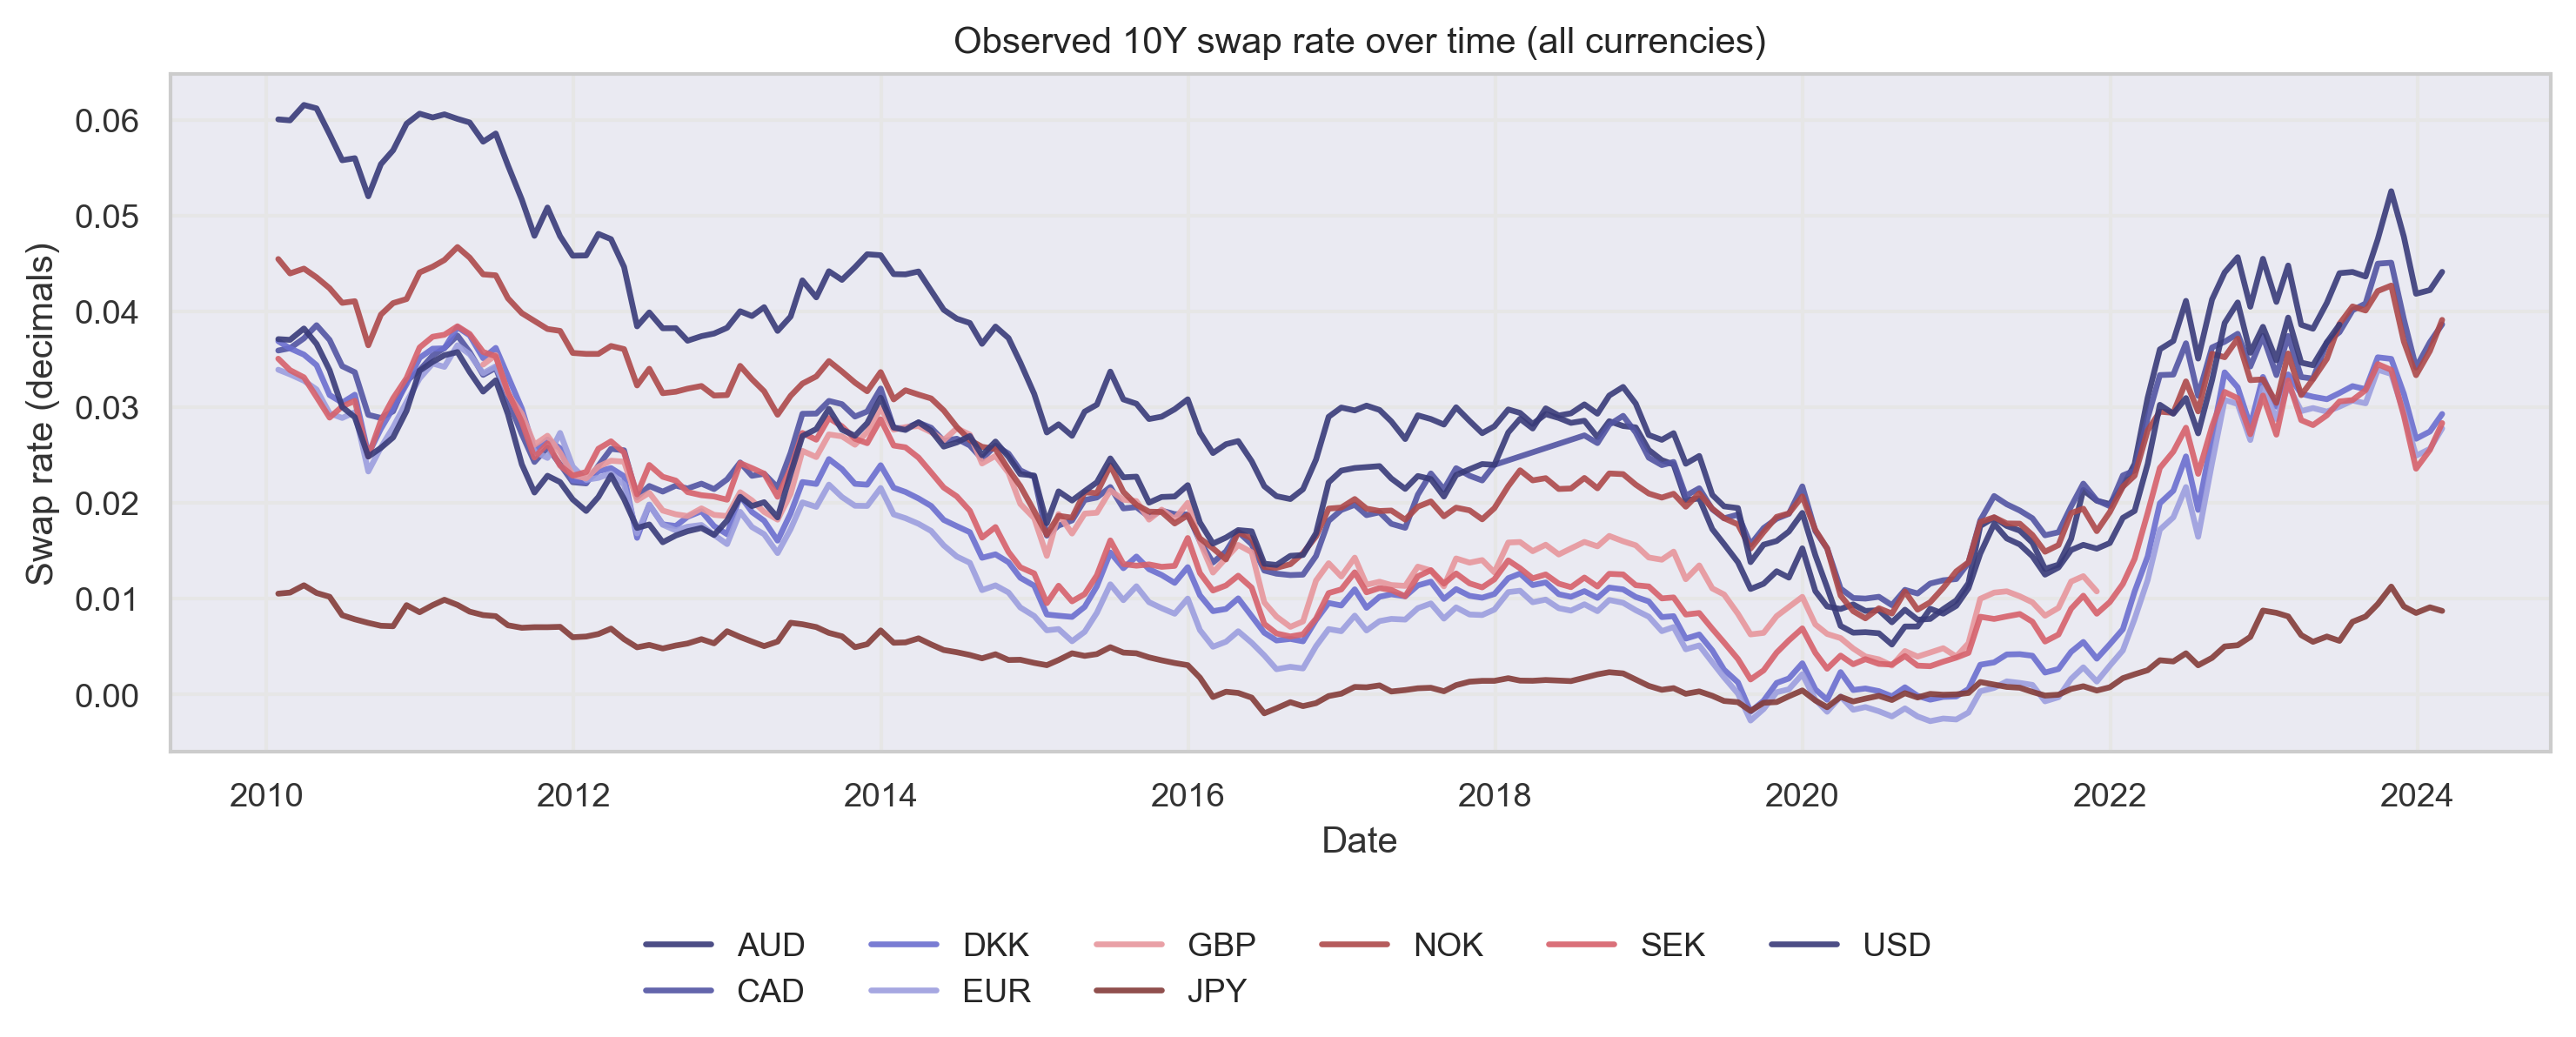
\includegraphics[width=0.9\textwidth]{Figures/bbg/paper_fig2b_timeseries_10_bbg.png}
    \caption{Time series of 10-year swap rates across currencies (2004--2024).}
    \label{fig:timeseries_10y}
\end{figure}

At the same time, the data display strong cross-currency comovement. Movements in Danish and euro swap rates are particularly close throughout the sample, while the Japanese series remains at a lower level and exhibits more muted variation for much of the period. More broadly, the figure suggests that global interest rate cycles affect all currencies, but with meaningful differences in level, volatility, and adjustment speed. This combination of common global movements and persistent cross-currency heterogeneity is important for the empirical analysis, since the model must be able to capture both shared structure and idiosyncratic curve behavior.

Overall, the dataset provides a demanding empirical setting for term structure modeling. It combines cross-sectional variation in curve shape, persistent differences across currencies, and substantial time-series variation across distinct interest rate regimes. These features make the sample suitable for evaluating whether the affine-inspired arbitrage-free encoder--decoder framework can fit observed swap curves consistently across currencies and over time.